
%%%%%%%%%%%%%%%%%%%%%%%%%%%%%%%%%%%%%%%%%
% Beamer Presentation
% LaTeX Template
% Version 1.0 (10/11/12)
%
% This template has been downloaded from:
% http://www.LaTeXTemplates.com
%
% License:
% CC BY-NC-SA 3.0 (http://creativecommons.org/licenses/by-nc-sa/3.0/)
%
%%%%%%%%%%%%%%%%%%%%%%%%%%%%%%%%%%%%%%%%%

%----------------------------------------------------------------------------------------
%	PACKAGES AND THEMES
%----------------------------------------------------------------------------------------

\documentclass{beamer}

\usepackage[czech]{babel}
\usepackage[utf8]{inputenc}

\usepackage{listings}
\usepackage{xcolor}
\usepackage{graphicx}

\lstdefinestyle{sharpc}{language=[Sharp]C, frame=lr, rulecolor=\color{blue!80!black}}
\setbeamertemplate{caption}[numbered]

\mode<presentation> {
    \usetheme{Copenhagen}
}

\usepackage{graphicx} % Allows including images
\usepackage{booktabs} % Allows the use of \toprule, \midrule and \bottomrule in tables

%----------------------------------------------------------------------------------------
%	TITLE PAGE
%----------------------------------------------------------------------------------------

\title{Metody statické analýzy malware} % The short title appears at the bottom of every slide, the full title is only on the title page
\author{Bc. Jan Hložek} % Your name

\institute[VŠB - TUO] % Your institution as it will appear on the bottom of every slide, may be shorthand to save space
{
\textit{prof. Ing. Ivan Zelinka, Ph.D.} \\
\medskip 
\medskip % Your email address 
Vysoká škola báňská – Technická univerzita Ostrava % Your institution for the title page

}
\date{25. června 2020}

\begin{document}

\begin{frame}
\titlepage % Print the title page as the first slide
\end{frame}

%%%%%%%%%%%%%%%%%%%%%%%%%%
\begin{frame}
\frametitle{Cíle práce} 

\begin{itemize}
    \item Rešerše aktuálního vědeckého poznání
    \item Analýza dané problematiky 
    \item Vytvoření vlastního řešení pro statickou analýzu
    \item Analýza malwaru
%\item Cil4
\end{itemize}

\end{frame}
%%%%%%%%%%%%%%%%%%%%%%%%%%
\begin{frame}
\frametitle{Aktuální stav vědeckého poznání} 

\begin{itemize}
    \item Využití strojového učení
    \item Limity statické analýzy
    \item Nové přístupy za použití obrazové analýzy
\end{itemize}

\centering
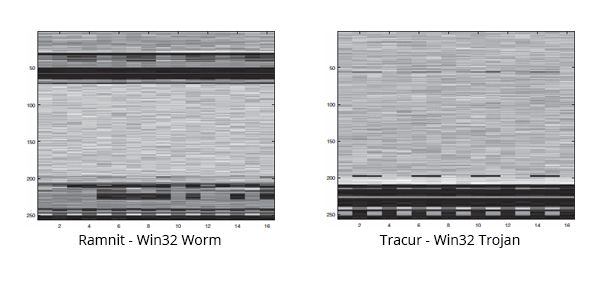
\includegraphics[width=0.8\textwidth]{images/obrazova-analyza.png}

\end{frame}
%%%%%%%%%%%%%%%%%%%%%%%%%%
\begin{frame}
\frametitle{Vlastní řešení} 

\begin{itemize}
    \item Nástroj pro automatizovanou statickou analýzu
    
    \begin{itemize}
        \item Návrh aplikace
        \item Využití externích knihoven
        \item Implementace vlastní knihovny a aplikací
    \end{itemize}
    
    \item Analýza výstupu statické analýzy pomocí strojového učení
\end{itemize}

\end{frame}


\begin{frame}
\frametitle{Vlastní řešení - schéma} 

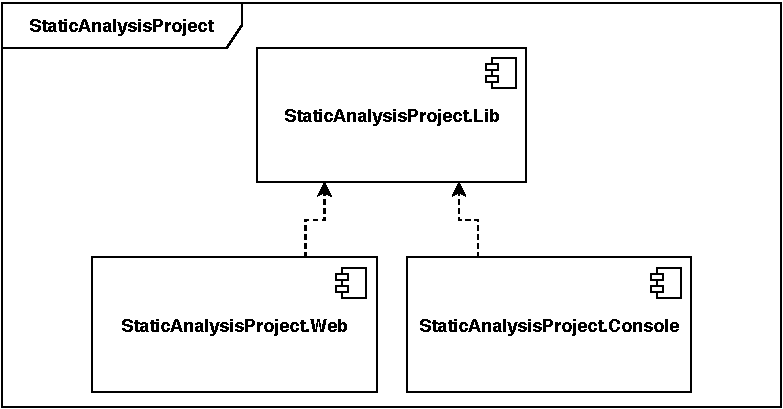
\includegraphics[width=\textwidth]{images/diagram-architektura.pdf}

\end{frame}


\begin{frame}
\frametitle{Vlastní řešení - vývoj} 

\hspace{5}

\begin{itemize}
    \item .NET standard - implementace knihovny
    \item .NET Core - konzolová aplikace
    \item ASP.NET Core - webová aplikace
\end{itemize}

\centering
\begin{picture}(250,250)
    \put(10,0){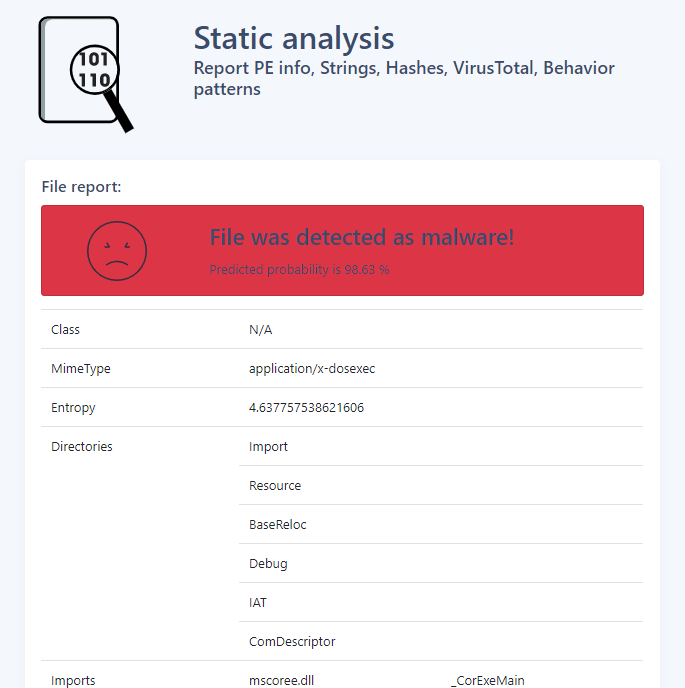
\includegraphics[width=0.75\textwidth]{images/web.png}}
\end{picture}

\end{frame}

\begin{frame}
\frametitle{Vlastní řešení - použité knihovny} 

\begin{itemize}
    \item VirusTotalNET - VirusTotal API
    \item Yara - detekce vzorů
    \item PeNET - analýza PE souboru
    \item MIME - detekce MIME typu
    \item ML.NET - strojové učení pro .NET
\end{itemize}

\centering
\begin{picture}(350,80)
    \put(40,0){
\includegraphics[width=0.75\textwidth]{images/knihovny.png}}
\end{picture}

\end{frame}

%\begin{frame}
%\frametitle{Vlastní řešení - výstup konzolové aplikace} 
%\centering
%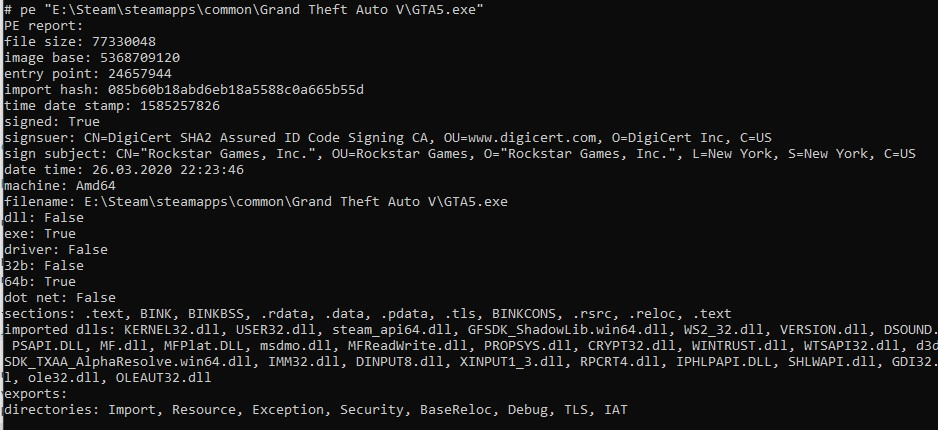
\includegraphics[width=\textwidth]{images/konzole-pe.jpg}
%\end{frame}
%\begin{frame}
%\frametitle{Vlastní řešení - výstup webové aplikace} 
%\centering
%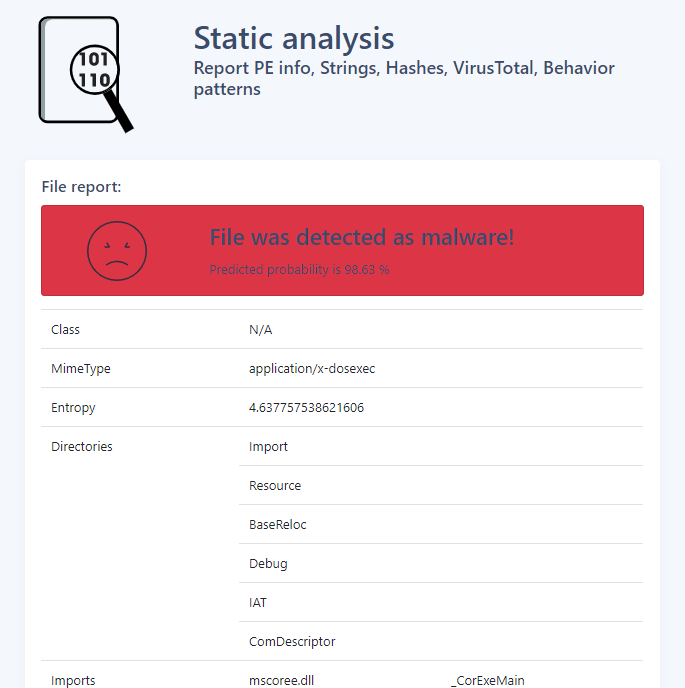
\includegraphics[width=90mm]{images/web.png}
%\end{frame}

\begin{frame}
\frametitle{Vlastní řešení - vytvoření databáze} 

\begin{itemize}
    \item Vytvoření datového setu 
    
    \begin{itemize}
        \item 1952 vzorků malwaru
        \item 108 legitimních aplikací
    \end{itemize}
    
    \item Použité databáze
        \begin{itemize}
            \item Github repositář ytisf/theZoo
            \item dasmalwerk.eu
        \end{itemize}
        
    \item Vytvoření a validace predikčního modelu v ML.NET
        \begin{itemize}
            \item Parametry PE (platforma, entropie atd.)
            \item Výstup analýzy řetězců (url, ip, soubory atd.)
            \item Detekována pravidla Yara
        \end{itemize}
\end{itemize}

\end{frame}

\begin{frame}
\frametitle{Vlastní řešení - testování} 

\begin{itemize}
    \item Vlastní malware (keylogger a bot)
    \item Malware databáze
        \begin{itemize}
            \item VirusShare.com
        \end{itemize}
    \item Legitimní aplikace
\end{itemize}

\begin{table}[]
    \centering
    
    \resizebox{0.85\textwidth}{!}{\begin{minipage}{\textwidth}
        \begin{tabular}{|l|l|l|l|l|}
            \hline
                            & Počet vzorků & Detekováno & Nedetekováno \\ \hline \hline
            Vlastní malware & 2            & 2          & 0     \\ \hline
            Ostatní malware & 20           & 20         & 0     \\ \hline
            Goodware        & 20           & 3          & 17    \\ \hline
        \end{tabular}
        
        \caption{Výsledky testování detekce malwaru}
    \end{minipage}}
\end{table}

\end{frame}

%%%%%%%%%%%%%%%%%%%%%%%%%%
\begin{frame}
\frametitle{Závěr}


\begin{itemize}

    \item V diplomové práci byla zpracována teoretická část pojednávající především o statické analýze a nových trendech jejího využití
    \item Na základě poznatků v teoretické části byl vytvořen program, který pomocí statické analýzy úspěšně detekuje malware
    \item Do budoucna by bylo vhodné hledat nové parametry, datovou kolekci doplnit o další vzorky, případně vytvořit vlastní knihovnu pro strojové učení

    %\item Použití statické analýzy pro detekování malwaru bylo úspěšné
    %\item Je potřeba dále hledat nové možnosti a parametry
    %\item Další rozšíření databáze o nové vzorky
\end{itemize}

\end{frame}

\begin{frame}
    \frametitle{}
    \centering \textbf{Děkuji za pozornost}
\end{frame}


\begin{frame}
\frametitle{Implementace vlastní knihovny pro strojové učení}

%https://machinelearningmastery.com/logistic-regression-for-machine-learning/

\begin{itemize}
\item Volba klasifikačního algoritmu
    \begin{itemize}
        \item Logistic regression
        %\item Decision tree
        \item kNN
    \end{itemize}
\item Transformace / normalizace vstupních dat (One-hot encoding)
\item Trénování modelu
\item Validace modelu (Cross-validation)
\item Klasifikace - predikování třídy
\end{itemize}

\end{frame}
\end{document} 